\documentclass[12pt]{article} % This command is used to set the type of document you are working on such as an article, book, or presenation

% \usepackage{geometry} % This package allows the editing of the page layout
% \usepackage{amsmath}  % This package allows the use of a large range of mathematical formula, commands, and symbols
% \usepackage{graphicx}  % This package allows the importing of images
\usepackage[T1]{fontenc}
\usepackage{blindtext}
\usepackage[]{algorithm2e}
\usepackage{graphicx}
\usepackage{float}
\usepackage{amsfonts, amssymb, amsmath}
\usepackage[utf8]{inputenc}
\usepackage{xcolor}
\usepackage{booktabs} % For better table lines
\usepackage{appendix} % For appendices
\usepackage{hyperref}
\hypersetup{
    colorlinks=true,
    linkcolor=blue,
    filecolor=magenta,      
    urlcolor=blue
    }

\parindent 0px

\graphicspath{ {../Assets} }

\title{Implementación de KDTree y KNN para clasificación de registros de datos de cardiopatías}
\date{septiembre 2023}
\author{Jesús Alpaca Rendón}     
\begin{document}
\maketitle
\section{Introducción}

El presente trabajo es para presentar una implementación de la estructura KDTree donde se insertaran los datos para después ser procesados
por K-Neighbords Nearest, esto ayuda a brindar una clasificación a los datos según su posición en el plano cartesiano. El algoritmo procesará
en esta ocasión datos de pacientes que fallecieron por causas del corazón, el registro tiene una lista de datos de diferentes características
donde indican si el paciente tuvo o no un ataque al corazón.
La idea principal es que se realice la experimentación de ver la exactitud que tiene el algoritmo para realizar correctamente la clasificación de datos

\section{Problema}

Se tiene una base de datos de pacientes que fallecieron por problemas en el corazón, aquí se muestra cuáles fallecieron por un ataque al corazón o como se diría comúnmente, infarto de miocardio y cuáles no.
El tamaño del conjunto de datos es de 1319 muestras, que tienen nueve campos, ocho de los cuales son de entrada y uno de salida. La edad,
el sexo (0 para mujer y 1 para hombre), la frecuencia cardiaca (impulso), la PA sistólica (presión alta), la PA diastólica (presión baja),
la glucemia (glucosa), la CK-MB (kcm) y la troponina (troponina) representan los campos de entrada, mientras que el campo de salida corresponde a la presencia
de infarto de miocardio (clase), que se divide en dos categorías (negativa y positiva); la negativa se refiere a la ausencia de infarto de miocardio, mientras que la positiva se refiere a la presencia de infarto de miocardio.
Se requiere tener un modelo que nos permita clasificar otros pacientes que puedan añadirse al registro de forma automática.
El dataset seleccionado se denomina "Heart Disease Classification Dataset", el cual se pudo verificar que con algoritmos de las librerias de python basadas en KNN, se obtuvo un accurance de 60 - 63 porciento, siendo otros algoritmos
más eficaces, sin embargo para el presente proyecto se realizara una implementación propia basada en el pseudocódigo de KDtree y KNN.

\section{KDTree y KNN}
\vspace{10mm}

KDTree
\vspace{10mm}

Es una estructura de datos que particiona el espacio en puntos organizados en k-dimensiones. Esta estructura de datos es muy util en aplicaciones de Machine Learning,
sin embargo si la cantidad de dimensiones que vaya procesando el KDTree, afecta la precisión de algoritmos de busqueda bastante. Uno de los metodos mas implementados en un KDTree
es el de Nearest Neighbord el cual encuentra el vecino mas cercano a un punto dado, y la forma de implementar este algoritmo se basa en como esta estructurado el arbol 
y en algunos casos la distancia del punto con el particionamiento que se dio al inicio.
\vspace{10mm}

KNN
\vspace{10mm}

K-Nearest Neighbords es un metodo de clasificación muy bueno que trabaja en valores basados en un array de datos de diferentes dimensiones, ya que principalmente se centra en 
hacer la comparativa de distancias con todos los puntos de una estructura, ordenar los resultados de menor a mayor y obtener los k vecinos mas cercanos al nodo a buscar.
Este algoritmo puede ser implementado sin problemas con una estructura de KDTree, tomando la ventaja del ordenamiento tan parejo que tiene la estructura, nos es facil reconocer los 
k vecinos cercanos a un nuevo nodo.
Hay diferentes formas de medir la distancia para puntos de n-dimensiones, en este caso se utilizo la distancia euclidiana, la cual esta formada por la siguiente formula:


\begin{figure}[H]
\centering
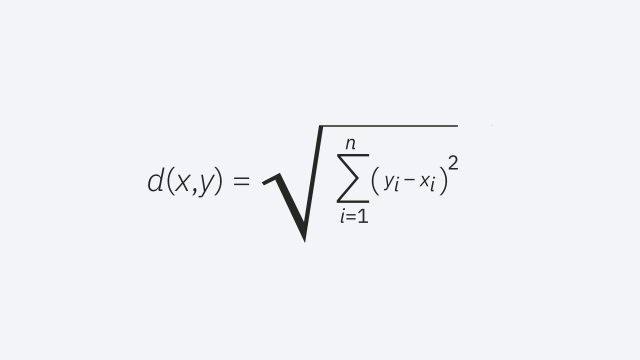
\includegraphics[width=\textwidth]{euclidiana}
\caption{Formula de distancia Euclidiana}
\end{figure}


\section{Implementación}
Para la implementacion se utilizo el lenguaje Python y la fuente de datos de Kaggle "Heart Disease Classification Dataset".
Adicionalmente se utilizaron librerias de python para la impresion de los graficos y el calculo de las metricas de medicion de los tests.
El link del repositorio es el siguiente:

- \href{https://github.com/Alpha004/AyEDJAAR2023/tree/main/Ejercicio_Final}{Repositorio Jesus Alpaca Rendon Ejercicio Final KDTree}

\section{Resultados}

La implementación ingresa los datos del dataset a la estructura del KDTree, después de ello, se aplica el KNN para encontrar los vecinos.
Para hacer la prueba correctamente, se obtuvo una serie de datos de test y datos de entrenamiento a partir del dataset principal para ejecutarlo
acorde a lo implementado.
El dataset contiene 1319 muestras de las cuales se utilizó la siguiente cantidad de datos para el entrenamiento y pruebas:

\begin{figure}[H]
\centering
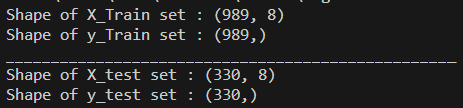
\includegraphics[width=\textwidth]{data}
\caption{Datos de Entrenamiento y Test}
\end{figure}

Se utilizó un total de 989 registros del dataset para entrenar la muestra y se utilizó 330 test para obtener
5 vecinos cercanos para cada uno, dando la clasificación a partir de la mayor cantidad de tipos de vecinos cercanos hallados.
Es decir, si 3 de 2 vecinos no tuvieron un ataque cardiaco, se clasifica con 0, que representa los pacientes que no tuvieron 
ningún tipo de ataque, y en caso contrario, se le marcara con 1.

Al ejecutar la implementación, se muestra la clasificación de data correcta y las predicciones que hallo el sistema:

\begin{figure}[H]
\centering
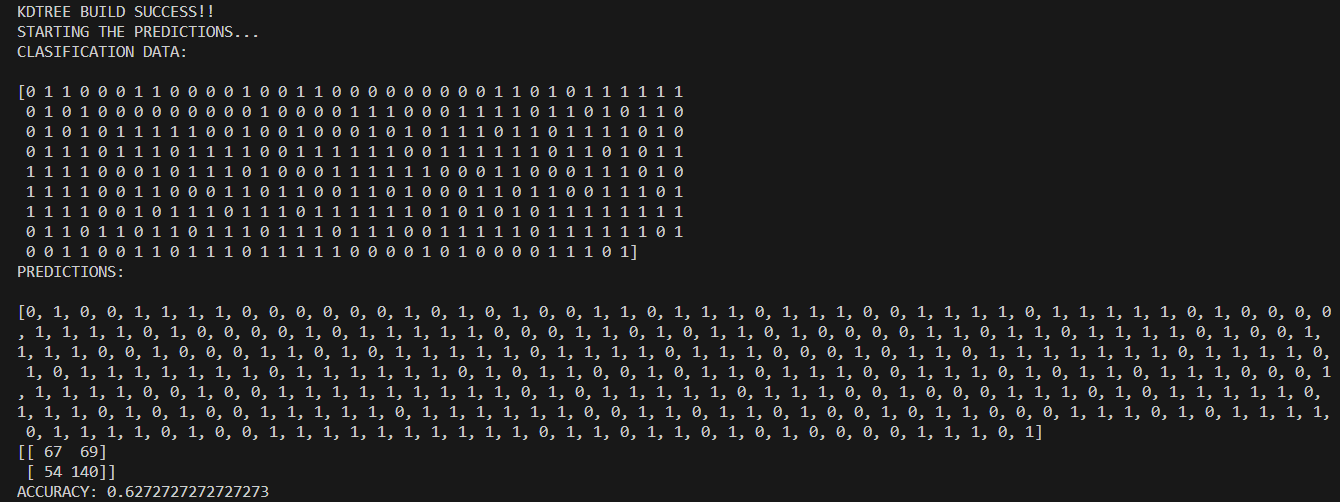
\includegraphics[width=\textwidth]{data2}
\caption{Clasificación y Predicciones}
\end{figure}

La matriz de comparación quedaría de la siguiente manera:

\begin{figure}[H]
\centering
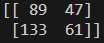
\includegraphics[width=\textwidth]{data3}
\caption{Matriz de comparación del test}
\end{figure}

Siendo el mismo orden con el que se representa la matriz en la teoria:

\begin{figure}[H]
\centering
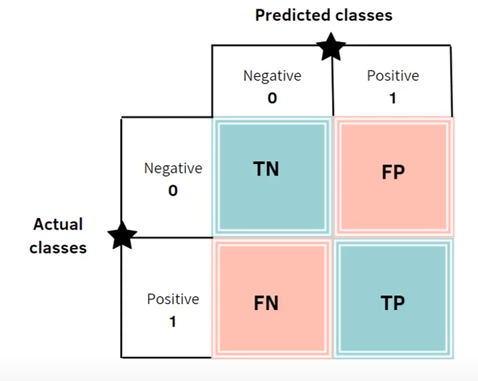
\includegraphics[width=\textwidth]{MatrizComparacion}
\caption{Matriz de comparación según la teoría}
\end{figure}

A partir de la tabla podemos empezar a sacar las métricas que nos indican cuanta precisión tendría nuestro modelo para clasificar:

\begin{figure}[H]
\centering
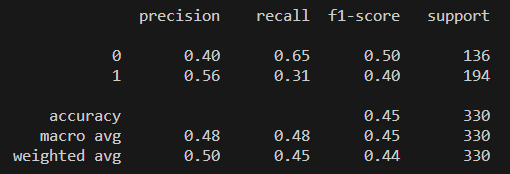
\includegraphics[width=\textwidth]{metricas}
\caption{Matriz de precisión de clasificación}
\end{figure}

Como se puede observar, se tiene una precisión promedio de 0.60 - 0.65, la cual está un poco alejada de una precisión aceptable para clasificación, incluso se podría decir que no es muy óptimo.
Esto debido a que el algoritmo de KNN en sí no tiene la precisión debida para darnos un resultado aceptable.

Podemos verificar uno de los resultados en los gráficos, como se indicó se tendría una gran cantidad de datos para el aprendizaje, por lo que se encontraran varios puntos en la gráfica.

\begin{figure}[H]
\centering
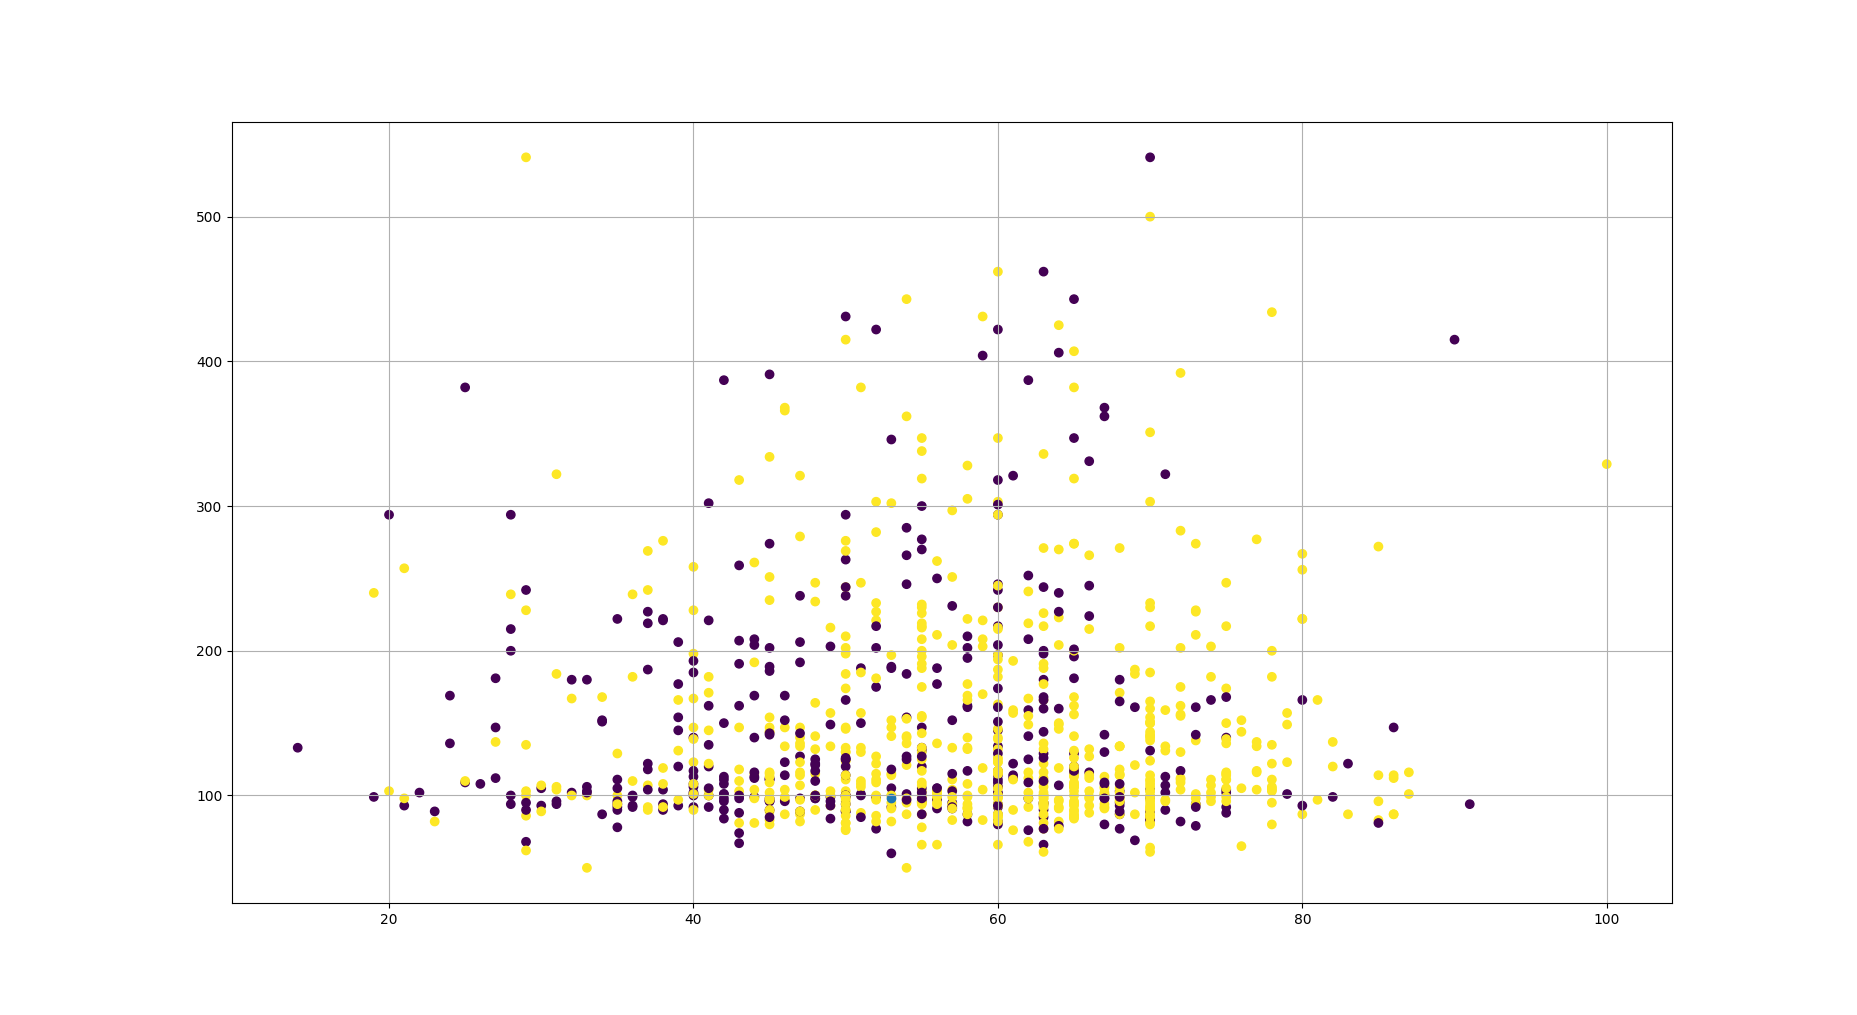
\includegraphics[width=\textwidth]{grafica1}
\caption{Gráfica de todos los puntos de training}
\end{figure}

Si nos acercamos más, podemos ver que el punto a clasificar, en este caso el punto azul, tiene 3 puntos amarillos, los cuales son de estado 0 y 2 morados de estado 1,
dando como resultado la clasificación a 0. Si revisamos los resultados mostrados en la figura 3, veremos que la predicción fue correcta.

\begin{figure}[H]
\centering
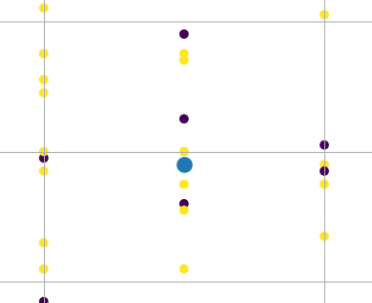
\includegraphics[width=\textwidth]{grafica3}
\caption{Clasificación del punto inicial de test}
\end{figure}


\section{Conclusiones}
Como conclusiones se puede indicar lo siguiente:

\begin{itemize}
    \item La implementación de KDTree para la resolución del problema es una investigación que denota interés, ya que es una de las estructuras multidimensionales más completas.
    \item Se debe considerar que la precisión obtenida no es muy aceptable ya que con mucho esfuerzo logra pasar el 50\% de precisión, KNN no seria un algoritmo idoneo para clasificar datos.
    \item Existen otros algoritmos mas fuertes que pueden aplicar una precisión mas aceptable, lo cual se recomienda realizar un proceso similar con otros algoritmos.
\end{itemize}

\begin{thebibliography}{9}
    \bibitem{libro1}
    Steinbach, Michael and Tan Pang-Ning. \textit{The Top Ten Algorithms in Data Mining}. University of Minnesota Twin Cities, 1st Edition chapter 8, 2009.

    \bibitem{sitioweb1}
    Ching (Chingis). KNN-python-implementation. URL: \texttt{https://chingisoinar.medium.com/}
    
    \bibitem{sitioweb2}
    M.C. Edgar Moyete (Moyete) - Canal de Machine Learning. URL: \texttt{https://www.youtube.com/@Moyetepython}

\end{thebibliography}

\end{document}